\chapter{Result and Discussion}
\section{Dataset Preparation}
After the selection of our Dataset which is IStego100K\cite{7}, now we need to further process this dataset. It was not feasible to train the model using all data at once. So, Initially we splitted the dataset into different batches. Each batch consisting of 40,000 images (20000 cover images and 20000 stego images). We tried to train the model using this subset of datset but there was mermory Limitation problem. We then reduced the batch size to 30,000 (15,000 cover images and 15,000 stego images), but still faced the same issue. Finally, we set the batch size to 20,000 (10,000 cover and 10,000 stego), which allowed the training process to proceed successfully. To split the dataset, we utilized a Microsoft PowerShell script, which splitted the dataset into the desired subsets and stored them in respective subfolders.\\
\section{Trainig the Ensemble Model}
Before training the model, it was necessary to identify the most suitable features for our project. Therefore, we conducted several tests to determine the optimal feature set for training our model.
\subsection{DCTR Feature}
Initially, we used (DCTR) features with a feature dimensionality of 8000 for training our model. However, we faced several challenges: the feature extraction process was time-consuming, and the outcomes were unsatisfactory.\\
\begin{figure}[H]
    \begin{subfigure}[b]{0.5\textwidth}
        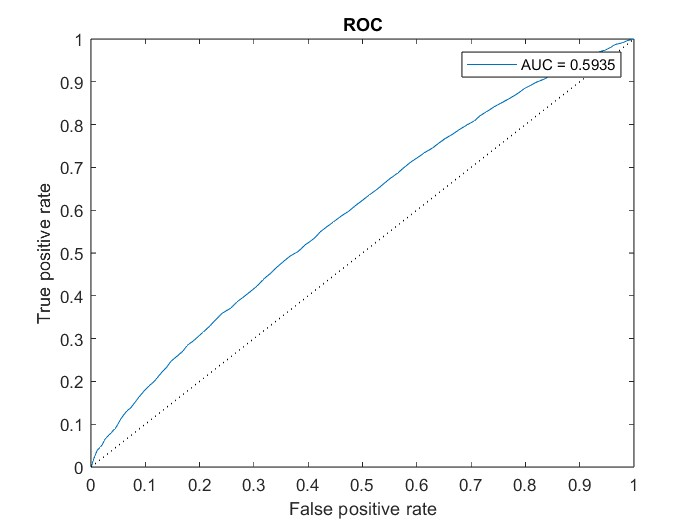
\includegraphics[width=\textwidth]{img/rocdctr.jpg}
    \end{subfigure}
    \hfill
    \begin{subfigure}[b]{0.5\textwidth}
        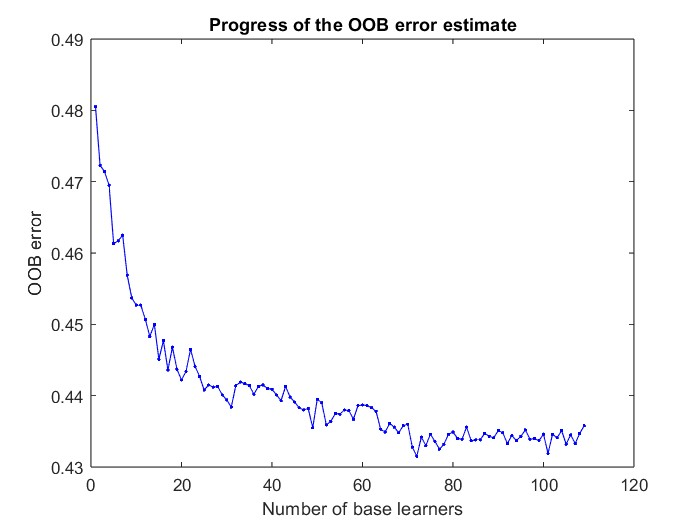
\includegraphics[width=\textwidth]{img/saturationdctr.jpg}
    \end{subfigure}
    \caption{ROC curve and OOB vs No of base learner [DCTR]}
\end{figure}
\begin{figure}[H]
    \begin{subfigure}[b]{0.5\textwidth}
        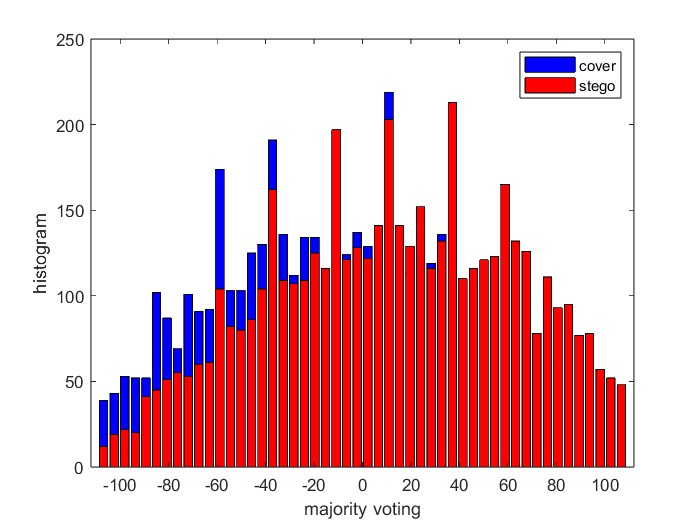
\includegraphics[width=\textwidth]{img/histoDctr.jpg}
    \end{subfigure}
    \hfill
    \begin{subfigure}[b]{0.5\textwidth}
        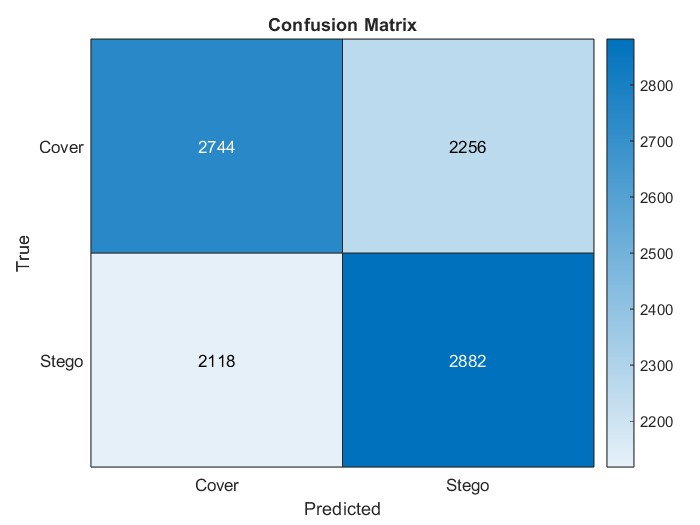
\includegraphics[width=\textwidth]{img/confusiondctr.jpg}
    \end{subfigure}
    \caption{Histogram and Confusion Matrix [DCTR]}
\end{figure}
\begin{flushleft}
Using DCTR as feacture vector for trainig the model we got Area Under the Curve (AUC) of 0.59 which is quite low. We tried using different sub-set of data set but result was still same. Above graphs shows ROC curve, OOB error vs number of base learner, confusion matrix and histogram of votes.
\end{flushleft}
\clearpage
\subsection{CC-CN Feature}
Later on, we came across cc-cN features, specifically cc-c300, which provided a higher dimensionality of 48600. These features proved to be more effective in capturing dependencies among individual cover elements. Due to the large dimensionality of our images, we used for Fisher's Linear Discriminant (FLD) as the base learner for our ensemble classifier. As a result, we observed improved performance compared to our earlier one.\\
\begin{figure}[H]
    \begin{subfigure}[b]{0.5\textwidth}
        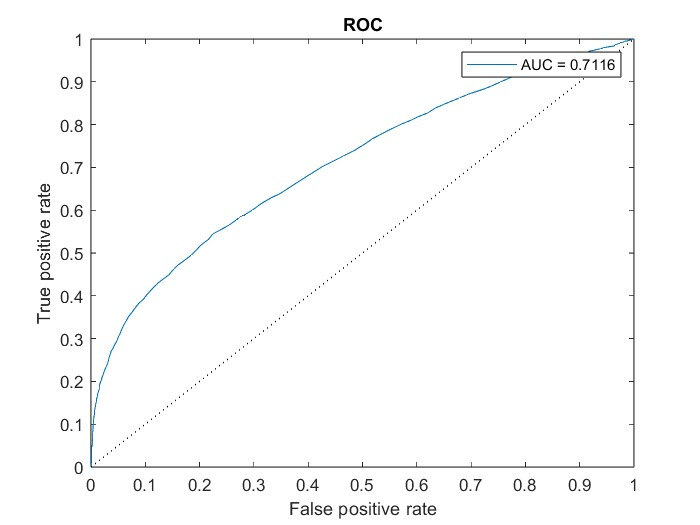
\includegraphics[width=\textwidth]{img/ROC300.jpg}
    \end{subfigure}
    \hfill
    \begin{subfigure}[b]{0.5\textwidth}
        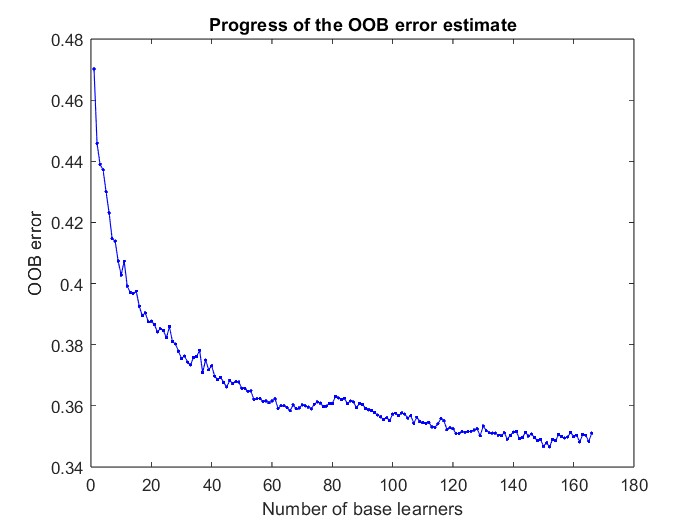
\includegraphics[width=\textwidth]{img/saturation300.jpg}
    \end{subfigure}
    \caption{ROC and Search for subspace dimensionality [CC-C300]}
\end{figure}
\begin{figure}[H]
    \begin{subfigure}[b]{0.5\textwidth}
        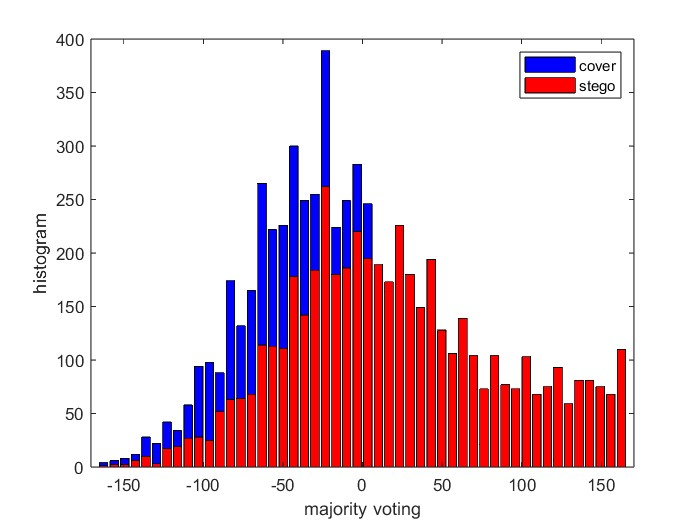
\includegraphics[width=\textwidth]{img/histo300.jpg}
    \end{subfigure}
    \hfill
    \begin{subfigure}[b]{0.5\textwidth}
        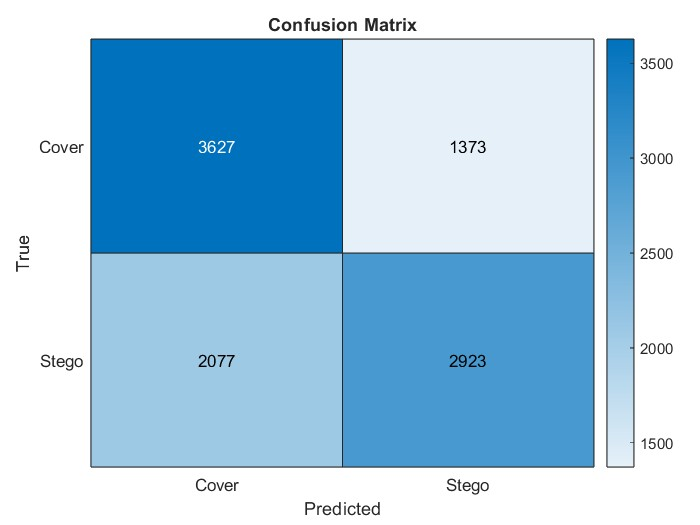
\includegraphics[width=\textwidth]{img/confusion300.jpg}
    \end{subfigure}
    \caption{Histogram and Confusion Matrix [CC-C300]}
\end{figure}
\begin{flushleft}
Above graphs shows ROC curve, OOB error vs number of base learner, confusion matrix and histogram of votes.Using CC-C300 as feature vector for training the model we got Area Under the Curve (AUC) of 0.7116 which is comparatively higher than the DCTR model. Upon using different sub-set of datasets the result was still same. The OOB error was minimum when number of base learners was 160.
\end{flushleft}
\clearpage
\subsection{CC-CHEN Feature}
We looked into another feature extraction method called cc-chen, which had 972 dimensions, to see if it was better than cc-c300. However, the results weren't as good as with cc-c300. So, we decided that cc-c300 was the best choice for our project.\\
\begin{figure}[H]
    \begin{subfigure}[b]{0.5\textwidth}
        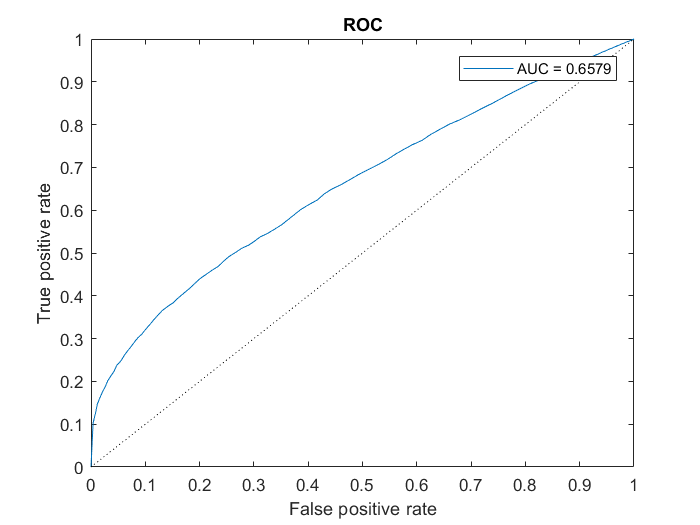
\includegraphics[width=\textwidth]{img/ROCchen.png}
    \end{subfigure}
    \hfill
    \begin{subfigure}[b]{0.5\textwidth}
        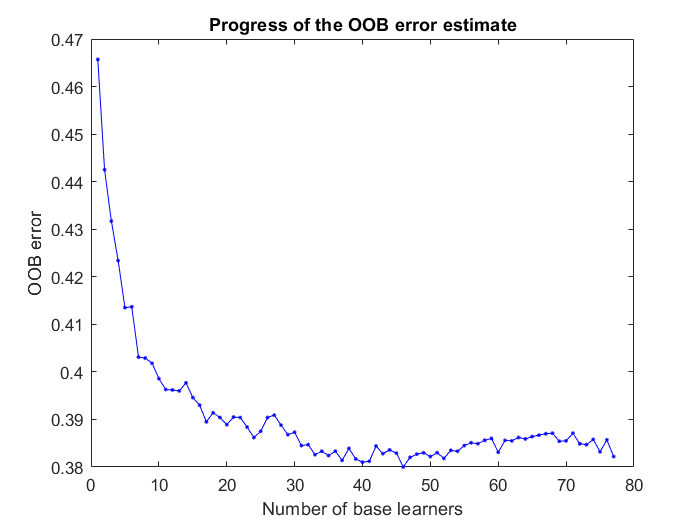
\includegraphics[width=\textwidth]{img/saturationchen.png}
    \end{subfigure}
    \caption{ROC and Search for subspace dimensionality [CC-CHEN]}
\end{figure}
\begin{figure}[H]
    \begin{subfigure}[b]{0.5\textwidth}
        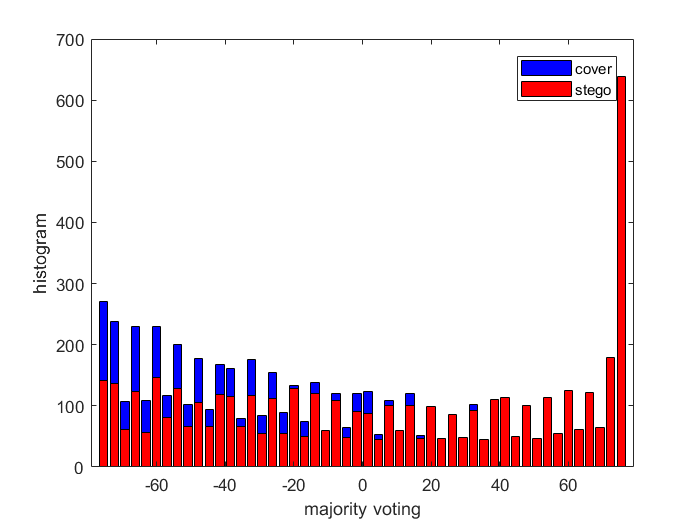
\includegraphics[width=\textwidth]{img/histochen.png}
    \end{subfigure}
    \hfill
    \begin{subfigure}[b]{0.5\textwidth}
        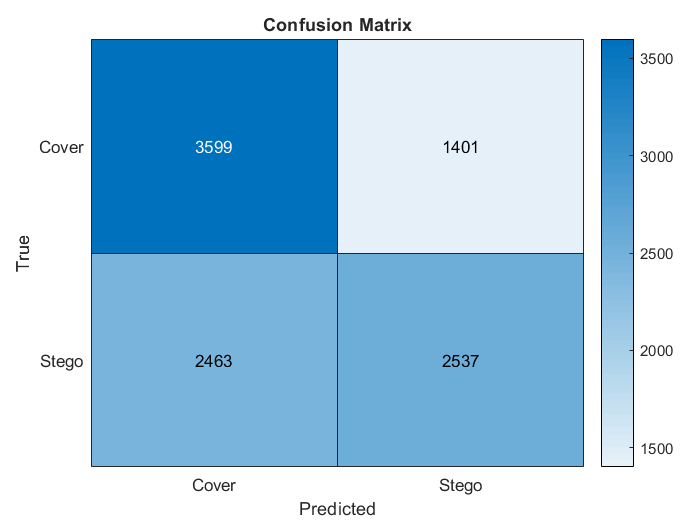
\includegraphics[width=\textwidth]{img/confusionChen.png}
    \end{subfigure}
    \caption{Histogram and Confusion Matrix [CC-CHEN]}
\end{figure}
\begin{flushleft}
Table below contiain summary of the performance of the model with different features.
\end{flushleft}
\begin{table}[H]
    \centering
    \begin{tabular}{|l|l|l|l|l|}
    \hline
    Feature & Accuracy & Precision & Recall & F1 Score \\ \hline
    DCTR    & 0.56   & 0.55    & 0.56 & 0.56  \\ \hline
    CC-CHEN & 0.61     & 0.70      & 0.59   & 0.65     \\ \hline
    CC-C300 & 0.66     & 0.73      & 0.64   & 0.68     \\ \hline
    \end{tabular}
    \caption{Performance of the model with different features}
\end{table}
\clearpage
\section{Changing different parameters}
After comparing with two other features we decied to choose CC-C300 feature. To get the optimal result we trained our model with different value of dsub and number of base learner. The results are shown below:
\begin{table}[H]
    \centering
    \begin{tabular}{|l|l|l|l|l|}
    \hline
    No of  Base Learner & Subspace size & Accuracy & Precision & Recall \\ \hline
    120                 & 800           & 0.6947   &    0.79       &  0.60      \\ \hline
    100                 & 1400         & 0.7045   &    0.64       &   0.62     \\ \hline
    160                 & 2600         & 0.7116   &    0.73       &    0.64    \\ \hline
    \end{tabular}
    \caption{Performance of the model with different parameters}
\end{table}

\begin{figure}[H]
    \begin{subfigure}[b]{0.5\textwidth}
        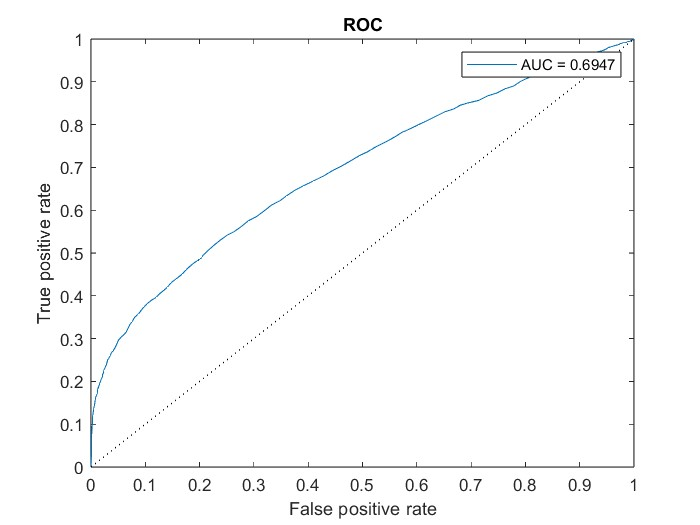
\includegraphics[width=\textwidth]{img/800/rocgray.jpg}
    \end{subfigure}
    \hfill
    \begin{subfigure}[b]{0.5\textwidth}
        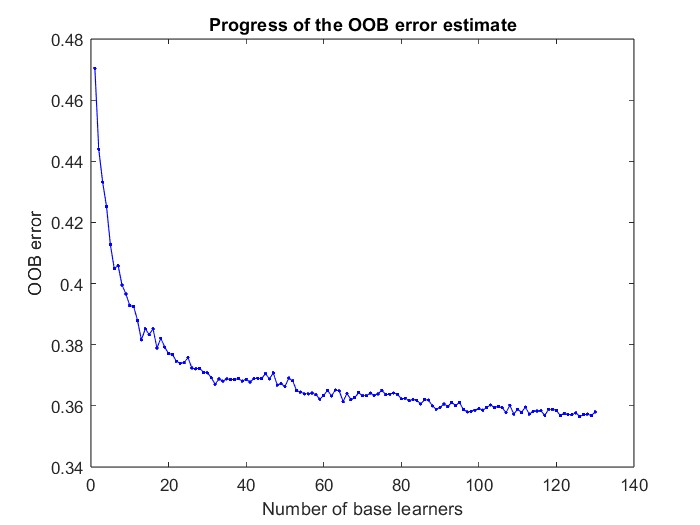
\includegraphics[width=\textwidth]{img/800/saturategray.jpg}
    \end{subfigure}
    \caption{ROC curve and OOB vs No of base learner[dsub=800]}
\end{figure}
\begin{figure}[H]
    \begin{subfigure}[b]{0.5\textwidth}
        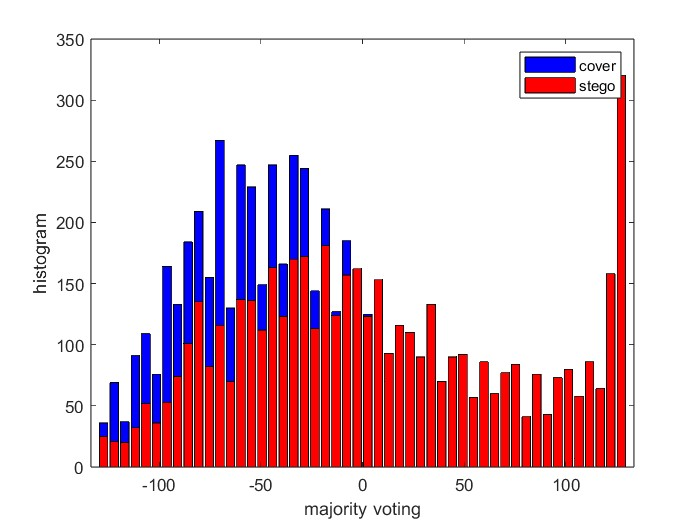
\includegraphics[width=\textwidth]{img/800/histogramgray.jpg}
    \end{subfigure}
    \hfill
    \begin{subfigure}[b]{0.5\textwidth}
        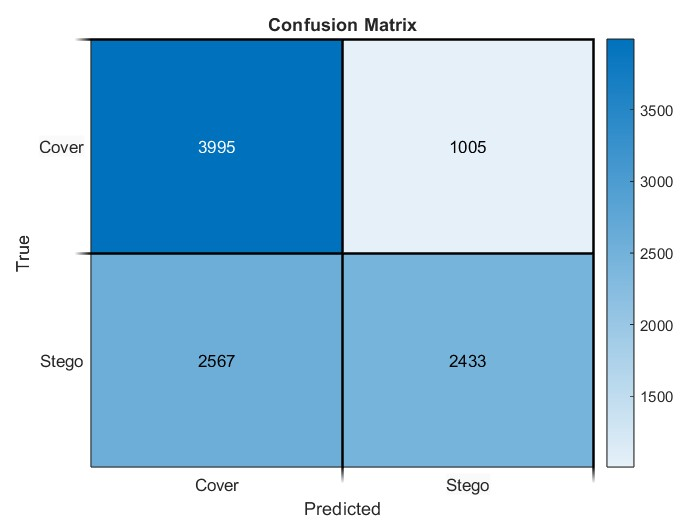
\includegraphics[width=\textwidth]{img/800/confusegray.jpg}
    \end{subfigure}
    \caption{Histogram and Confusion Matrix [dsub=800]}
\end{figure}
Using 800 sub space dimensionality with CC-C300 feature vector we got Area Under the Curve (AUC) of 0.69. The ROC curve, OOB error vs number of base learner, confusion matrix and histogram of votes are shown in the above graphs. The OOB error was minimum when number of base learner was 120. In this process we made sub space dimensionality constant of 800 while number of base learner to automatically get selected when OOB error was minimum.

\begin{figure}[H]
    \begin{subfigure}[b]{0.5\textwidth}
        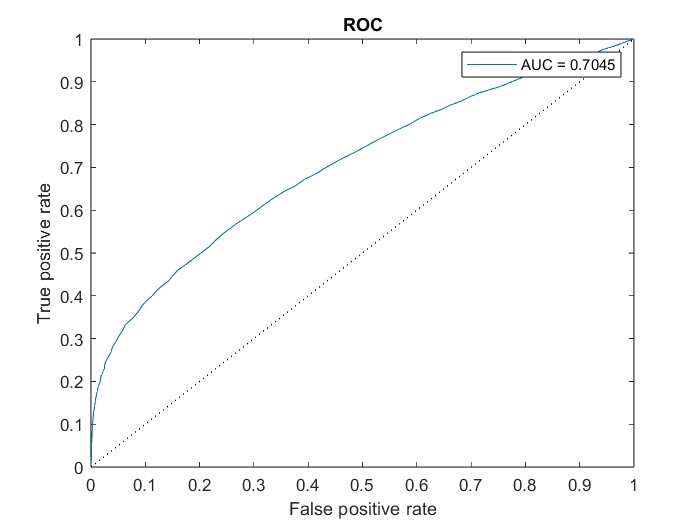
\includegraphics[width=\textwidth]{img/1400/gray1400roc.jpg}
    \end{subfigure}
    \hfill
    \begin{subfigure}[b]{0.5\textwidth}
        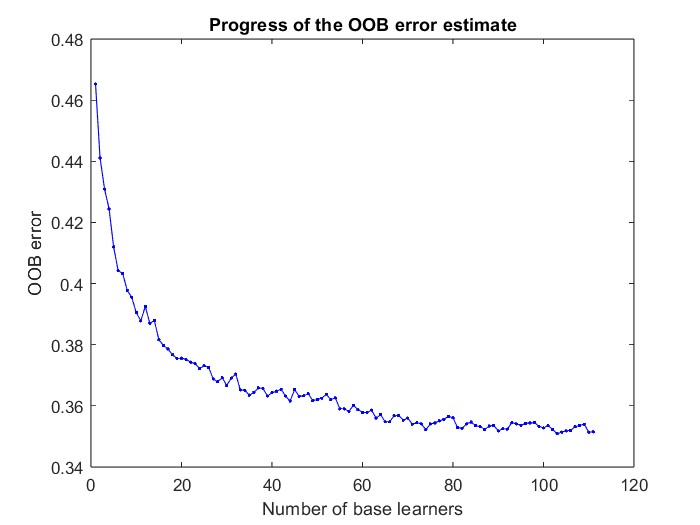
\includegraphics[width=\textwidth]{img/1400/gray1400saturate.jpg}
    \end{subfigure}
    \caption{ROC curve and OOB vs No of base learner [dsub=1400]}
\end{figure}
\begin{figure}[H]
    \begin{subfigure}[b]{0.5\textwidth}
        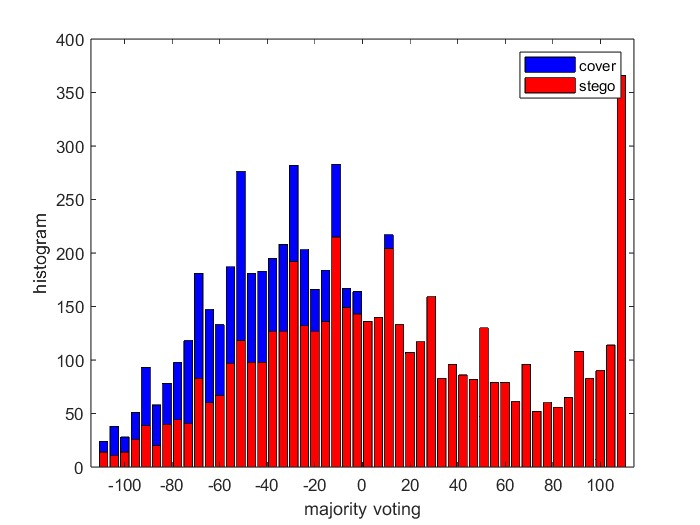
\includegraphics[width=\textwidth]{img/1400/gray1400histo.jpg}
    \end{subfigure}
    \hfill
    \begin{subfigure}[b]{0.5\textwidth}
        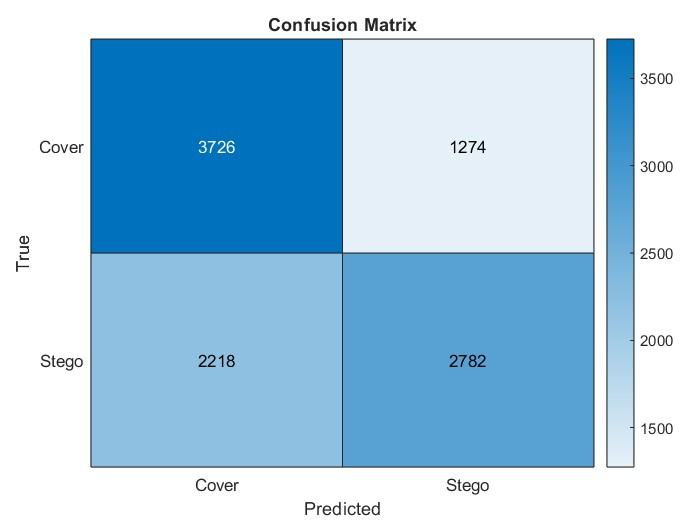
\includegraphics[width=\textwidth]{img/1400/gray1400confuse.jpg}
    \end{subfigure}
    \caption{Histogram and Confusion Matrix [dsub=1400]}
\end{figure}
After that we changed sub space dimensionality to 1400, we examined a model's performance and got an Area Under the Curve (AUC) of 0.7045. ROC curves, OOB error versus the number of base learners, a confusion matrix, and a vote histogram were used to illustrate the behavior of the model. The least amount of out-of-bag error (OOB) was obtained when 100 base learners were used. In order to reduce the OOB error, the number of base learners was automatically adjusted during the analysis, with the subspace dimensionality fixed at 1400.
\begin{figure}[H]
    \begin{subfigure}[b]{0.5\textwidth}
        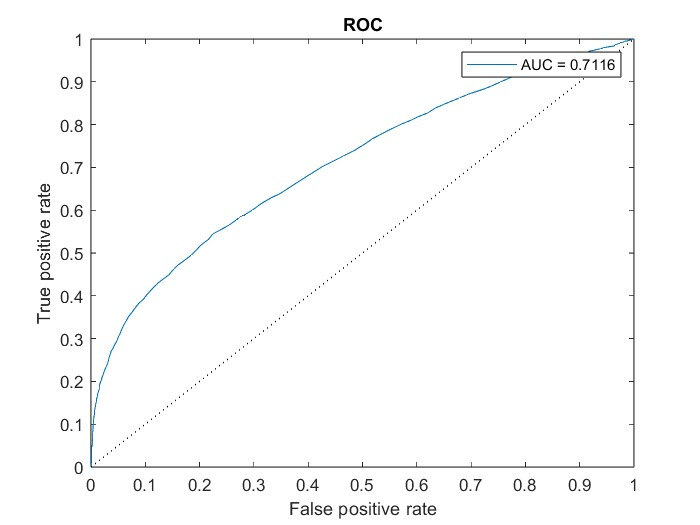
\includegraphics[width=\textwidth]{img/2600/roc2600.jpg}
    \end{subfigure}
    \hfill
    \begin{subfigure}[b]{0.5\textwidth}
        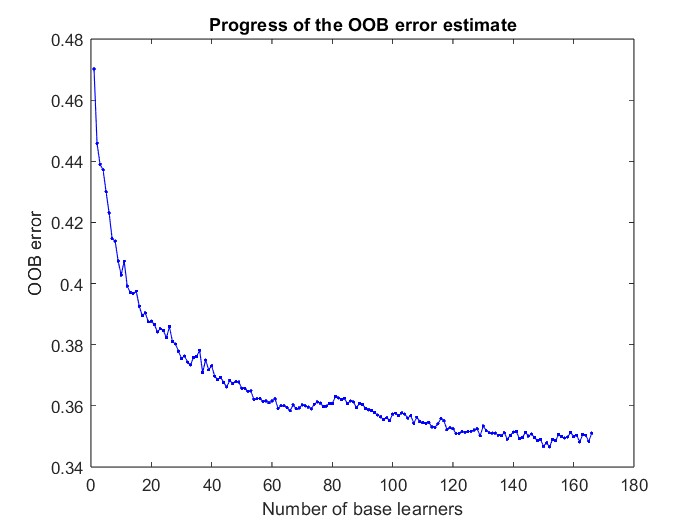
\includegraphics[width=\textwidth]{img/2600/staturAATE2600.jpg}
    \end{subfigure}
    \caption{ROC curve and OOB vs No of base learner[dsub=2600]}
\end{figure}
\begin{figure}[H]
    \begin{subfigure}[b]{0.5\textwidth}
        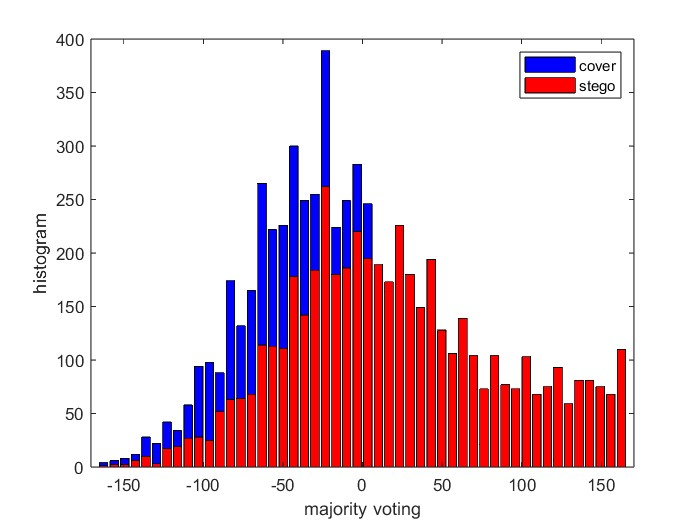
\includegraphics[width=\textwidth]{img/2600/histo2600.jpg}
    \end{subfigure}
    \hfill
    \begin{subfigure}[b]{0.5\textwidth}
        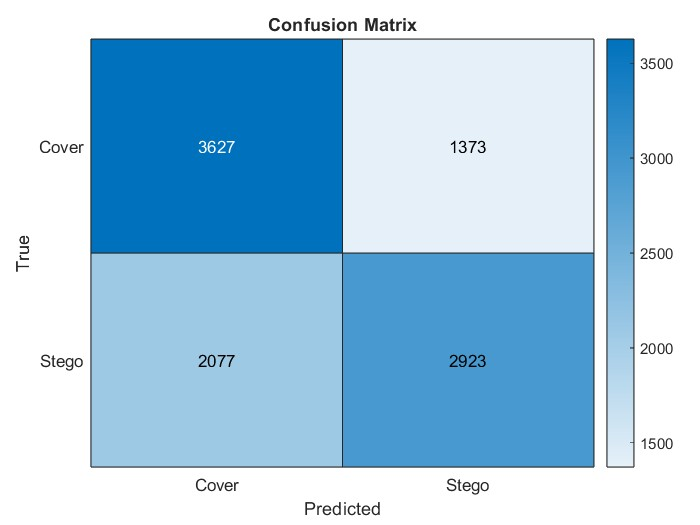
\includegraphics[width=\textwidth]{img/2600/consuse2600.jpg}
    \end{subfigure}
    \caption{Histogram and Confusion Matrix [dsub=2600]}
\end{figure}
Using CC-C300 feature vectors and 2600 subspaces, we examined a model's performance. With an Area Under the Curve (AUC) of 0.7116. ROC curves, OOB error versus the number of base learners, a confusion matrix, and a vote histogram were used to illustrate the behavior of the model. The least amount of out-of-bag error (OOB) was obtained when 150 base learners were used. In order to reduce the OOB error, the number of base learners was automatically adjusted during the analysis, with the subspace dimensionality fixed at 2600.
\clearpage

\section{Comparison between MATLAB and Python}
The decision between MATLAB and Python as our primary platform was influenced by the availability of feature extraction tools. Since our feature extraction process was exclusive to MATLAB, we were inclined to opt for MATLAB. Although the functionality to call and use python engine inside MATLAB is available but there are limitations to their usage as there are version compatibility issues. For the functionality of using python in MATLAB we require matlabengine which has various bugs and they have various version compatibility issues as well.\\
There are also various procedure which had to be carefully followed in order to properly execute python libraries. 
Thus, although it’s possible to call MATLAB functions from Python, limitations such as version compatibility and slower execution using MATLAB Engine prompted us to stick with MATLAB for feature extraction\\
For the creation of the demos, there were functionalities to create app demo using MATLAB as backend and frontend as well but it required matlabengine which had as afore mentioned various compatibility issues. So, we opted to use MATLAB's matlab app designer functionality for creating a demo app without the need of matlabengine.






% In assessing classification methods, we experimented with using a Random Forest ensemble classifier in Python. The model's performance and accuracy closely matched those obtained using MATLAB.\\

% The decision between MATLAB and Python as our primary platform was influenced by the availability of feature extraction tools. Since our feature extraction process was exclusive to MATLAB, we opted for it. Although it's possible to call MATLAB functions from Python, limitations such as version compatibility and slower execution using MATLAB Engine prompted us to stick with MATLAB for feature extraction.\\
% TO call matlab from python it requires matlabengine. matlabengine is bla bla matlab ko version anusar python ko version vary garna parcha........ \\

% For creating a demo, we investigated using MATLAB as a backend. It was possible but again it rquired matlabengine. so we used matlab app designer for the UI. mmatlab app designer is bla bla bla
% k chutyo?
% about matlab Engine
% about matlab app designer
% why matlab engine not used---------> slower
% why matlab app designer used-----------> backend ma matlab engine use hune vayera 


\section{Result}
The following are the findings or results obtained from the selected model:
\subsection{Time requirements}
Table below shows the different time requirements for our project:
\begin{table}[H]
    \begin{tabular}{|l|l|}
    \hline
    S.N                & Average Time Required \\ \hline
    Feature Extratoion & 0.8 second per Image            \\ \hline
    Model Training with 20,000 images  & 10 minutes            \\ \hline
    Testing            & 30 second             \\ \hline
    \end{tabular}
    \caption{Time Requirements}
    \end{table}
\subsection{ROC Curve}
\begin{figure}[H]
    \centering
    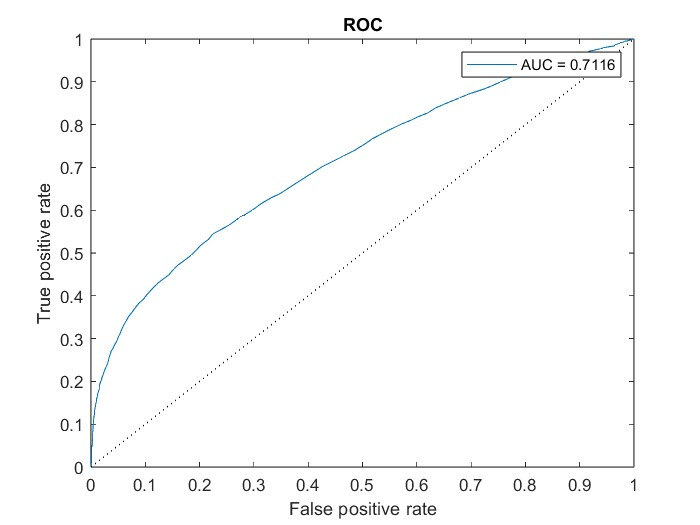
\includegraphics[width=120mm]{./img/2600/roc2600.jpg}
    \caption{ROC Curve}
\end{figure}
The ROC curve is a graphical representation of the contrast between true positive rates and the false positive rate at various thresholds. It is often used as a proxy for the trade-off between the sensitivity and the specificity of the model. The AUC is the area under the ROC curve. The higher the AUC, the better the performance of the model at distinguishing between the positive and negative classes.\\
We obtained Area Under the Curve (AUC) of 0.7116, indicating a high level of classification between positive and negative instances
\subsection{OOB Vs L}
\begin{figure}[H]
    \centering
    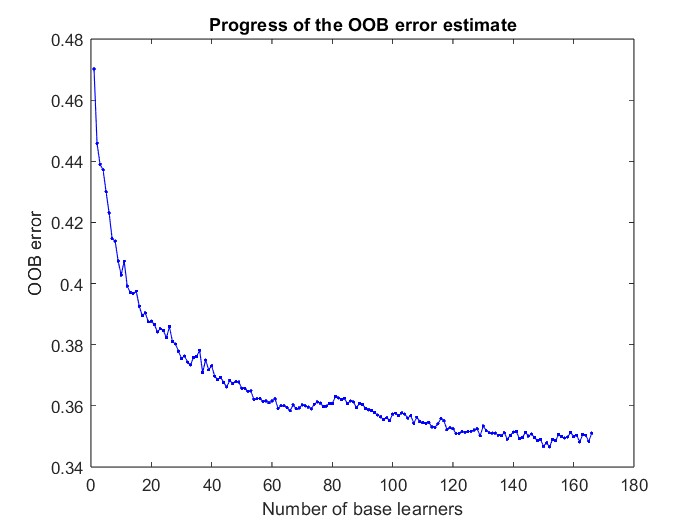
\includegraphics[width=120mm]{./img/2600/staturAATE2600.jpg}
    \caption{OOB Vs Number of Base Learners}
\end{figure}
Above graph shows different values of OOB error for different number of base learners. It is observed that the OOB error decreases as the number of base learners increases. The OOB error is minimum when the number of base learners is 160.
\subsection{Confusion Matrix}
\begin{table}[H]
\begin{figure}[H]
    \centering
    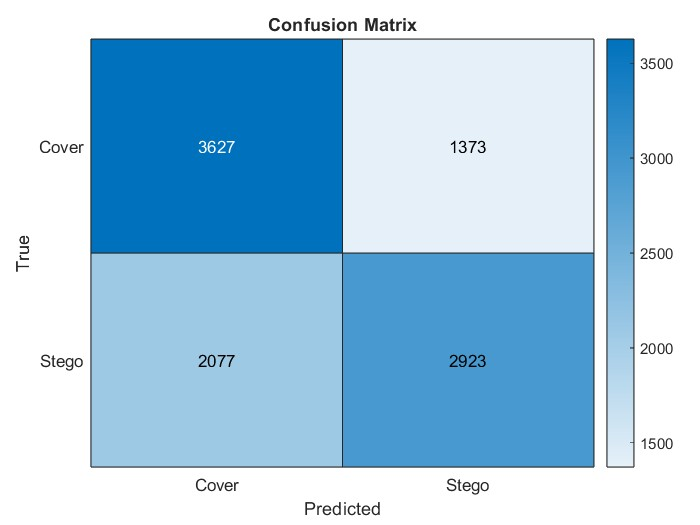
\includegraphics[width=120mm]{./img/2600/consuse2600.jpg}
\end{figure}
\caption{Confusion Matrix}
\end{table}
The model's classification performance is summarized through a confusion matrix, featuring 3627 true positives (correctly identified positives), 2923 false negatives (misclassified negatives), 2077 false positives (incorrectly labeled positives), and 1373 true negatives (correctly identified negatives). These metrics offer a concise yet comprehensive overview of the model's ability to distinguish between positive and negative cases, providing crucial insights for evaluating its effectiveness. The confusion matrix serves as a pivotal tool in assessing the model's strengths and weaknesses, contributing valuable information to the ongoing discourse on classification model refinement.
\subsection{Histogram}
\begin{figure}[H]
    \centering
    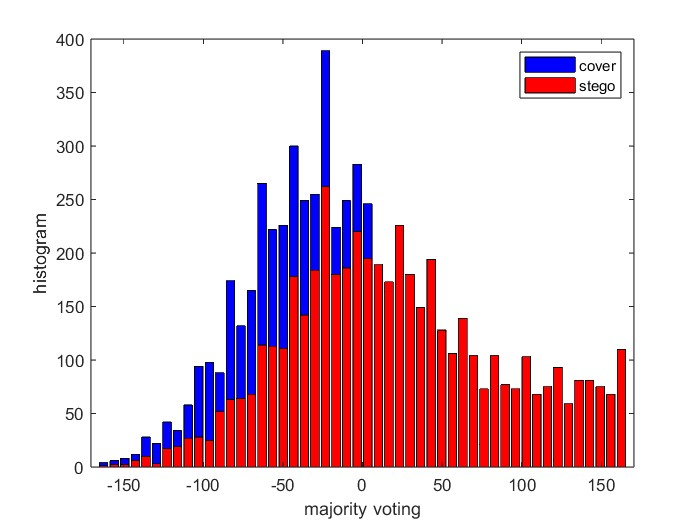
\includegraphics[width=120mm]{./img/2600/histo2600.jpg}
    \caption{Histogram of votes}
\end{figure}
The histogram of votes is a graphical representation of the number of votes for each class. The histogram provides a visual representation of the model's classification performance, offering insights into the distribution of votes across the different classes. The histogram is a valuable tool for evaluating the model's classification performance, providing a comprehensive overview of the distribution of votes and the model's ability to distinguish between positive and negative cases.

\section{Model Evaluation}
\subsection{Performance Metrices}
\subsection*{Precision}
Precision which is also called positive predictive value is the fraction of retrieved instances that are relevant. It is the ratio of true positive to the sum of true positive and false positive. It is given by the formula:
$$Precision = \frac{TP}{TP+FP} = \frac{3627}{3627+1373} = 0.73 $$
\subsection*{Accuracy}
Accuracy is the ratio of correctly predicted observation to the total observations. It is given by the formula:
$$Accuracy = \frac{TP+TN}{TP+TN+FP+FN}= \frac{3627+1373}{3627+1373+2077+2923}=0.66$$
\subsection{Recall}
Recall which is also called sensitivity is the fraction of relevant instances that have been retrieved over the total amount of relevant instances. It is the ratio of true positive to the sum of true positive and false negative. It is given by the formula:
$$Recall = \frac{TP}{TP+FN} = \frac{3627}{3627+2077}= 0.64$$
\subsection{F1 Score}
F1 Score is the weighted average of Precision and Recall. It is given by the formula:
$$F1\ Score = 2*\frac{Precision*Recall}{Precision+Recall} = 2*\frac{0.73*0.64}{0.73+0.64} = 0.68$$






